\chapter{Engenharia de Software}
\label{chap:engenharia}

\section{Introdução}
\label{engenharia:sec:introducao}
Neste capítulo irá ser descrito o planeamento da implementação do projeto, e decisões tomadas antes de qualquer desenvolvimento, sendo o facto de se planear implementar um sistema distribuído ao invés de 
apenas concorrente o fator que mais influenciou essas decisões.
Estas decisões incluem a Linguagem usada na Implementação, o método usado para testar o funcionamento da implementação,
o método de comunicação entre os Nós visto que se optou por um implementação distribuída e o modelo do sistema.

\section{Sistema Distribuído}
\label{engenharia:sec:sistema}
Como referido no capítulo \ref{chap:introducao}, a proposta inicial consistia em simular o protocolo num único programa,
mas o desenvolvimento de um sistema distribuído 
provaria-se uma implementação de maior interesse do algoritmo e ``fiel'', pois o \acs*{ADDP} foi desenvolvido para esse mesmo contexto.

Também foi ponderada a utilização de uma linguagem que fornecesse comunicação por canais,
visto que seria a noção mais próxima da comunicação entre os \emph{Nodes} tal como foi definida no \emph{paper} de referência, na qual se
escolheu a Linguagem \emph{Go} (ver \label{implementacao:subsec:go}), pois seria necessária a comunicação entre vários \emph{Threads}, estes simulando \emph{Nodes}.
No entanto, devido à alteração do contexto da implementação de Concorrente para Distribuído, não foi possível fazer uso deste tipo de canais, 
e optou-se por usar outra tecnologia que garantisse a comunicação remota entre os vários \emph{Nodes}.


\section{Linguagem Go}
\label{engenharia:sec:go}

A linguagem \emph{Go} facilita o desenvolvimento de sistemas concorrentes, pois, nativamente, oferece várias ferramentas para o desenvolvimento deste tipo de sistema.

Adicionando a palavra ``\emph{go}'' antes de qualquer procedimento, esse procedimento irá correr em uma nova \emph{Goroutine},
de forma concorrente em relação a todas as outras \emph{Goroutines} já em execução.
Uma ``Goroutine'' é um \emph{lightweight \textbf{thread}} gerida pelo \emph{runtime} do \emph{Go}.

Por exemplo, comparando (parcialmente) dois programas concorrentes, um em \emph{Go} e outro em \emph{Java}, que mostram os números inteiros de 0 a 10:
\begin{lstlisting}[caption={Exemplo em \emph{Go}, usando a \emph{keyword} ``go'' para começar uma \emph{Goroutine}.},language=Go]
func main() {
	var wg sync.WaitGroup
	wg.Add(2)
	go count(&wg, "Goroutine-1")
	go count(&wg, "Goroutine-2")

	wg.Wait()
}

func count(wg *sync.WaitGroup, goroutineName string) {
	defer wg.Done()
	for i := 0; i < 10; i++ {
		fmt.Printf("Thread %s, %d\n", goroutineName, i)
		time.Sleep(time.Second * 40)
	}
}
\end{lstlisting}


\begin{lstlisting}[caption={Exemplo em \emph{Java}, usando a \emph{interface} ``Runnable'' e uma classe``RunnableDemo'' para começar \emph{threads}.},language=Java]
class RunnableDemo implements Runnable {
   private Thread t;
   private String threadName;

   RunnableDemo( String name) {
      threadName = name;
   }
   public void run() {
      try {
	 for(int i = 10; i < 10; i++) {
	    System.out.println("Thread: " + threadName + ", " + i);
	    Thread.sleep(40);
	 }
      } catch (InterruptedException e) {
	 System.out.println("Thread " +  threadName + " interrupted.");
      }
   }
   public void start () {
      if (t == null) {
	 t = new Thread (this, threadName);
	 t.start ();
      }
   }
}

public class TestThread {

   public static void main(String args[]) {
      RunnableDemo R1 = new RunnableDemo("Thread-1");
      R1.start();

      RunnableDemo R2 = new RunnableDemo("Thread-2");
      R2.start();
   }   
}
\end{lstlisting}

Além da simplicidade na especificação de procedimentos concorrentes, a linguagem oferece bibliotecas nativas de apoio a programas concorrentes,
como a biblioteca ``sync'' que disponibiliza primitivas de sincronização simples 
(como por exemplo \emph{WaitGroups} e \emph{Mutex Locks}), e canais que permitem a comunicação e partilha de dados entre \emph{Goroutines}.

A concorrência é inerente aos sistemas distribuídos, visto que os vários elementos do sistema executam de forma independente e em simultâneo.

Um exemplo relacionado com o tema deste projeto seria o caso em que um \emph{Node} recebe vários pedidos de outros \emph{Nodes}.
De forma a manter o sistema (ou o diretório) consistente,
o \emph{Node} que recebe os pedidos terá de os tratar de forma sincronizada, isto é, tem de endereçar um pedido de cada vez.

Na implementação fez-se uso de servidores e pedidos \acs{HTTP} (ver \ref{engenharia:sec:comunicação}) que, por omissão,
todos os pedidos \acs{HTTP} que o servidor recebe são tratados em \emph{goroutines} diferentes,
de forma concorrente, o que permite a receção de vários pedidos e 
para a sincronização das \emph{goroutines} usou-se um ``Mutex'' proveniente da biblioteca ``sync''.





\section{Visualização do Sistema}
Foi decidida a implementação de uma visualização do sistema. 
Esta visualização permitiria a testagem da programa durante a implementação do sistema,
tornaria mais fácil a compreensão do funcionamento do sistema e possivelmente provar o seu bom funcionamento.

Surgiram várias hipótese de implementação, como a utilização de bibliotecas de bibliotecas gráficas para desenvolver a interface de visualização,
no entanto o suporte destas bibliotecas na Linguagem \emph{Go} não era o desejado, ficando então decidido o uso de uma página \emph{Web}.

Mesmo que a atualização da interface numa página \emph{Web} não fosse tão eficiente como a de uma biblioteca gráfica, esta provou-se útil 
pelo facto de ser possível aceder a esta interface fora do sistema, isto é, sem ser necessário que uma das máquinas do sistema distribuído possuísse 
um monitor, e também garantindo o acesso remoto a esta mesma visualização.

\subsection*{\emph{JavaScript}}
Para a implementação da visualização foi usado \textbf{JavaScript}.
Esta linguagem permite que a informação de páginas \emph{Web} seja alterada após o seu carregamento.
É usado no desenho de grafos e alteração de tabelas que dispõem a informação da visualização da rede.

\section{Comunicação entre os \emph{Nodes}}
\label{engenharia:sec:comunicação}
Como referido em na secção \ref{engenharia:sec:sistema}, o facto de se ter planeado implementar um sistema distribuído
em vez de um programa concorrente, tornou-se impossível o uso de comunicações por canais do \emph{Go}, 
e para a comunicação seria necessário um método de comunicação por rede.

Inicialmente procurou-se reproduzir o conceito de comunicação por canais da linguagem \emph{Go}, mas que esta fosse por rede, ou seja, algo que possivelmente
usa-se uma sintaxe ou conceitos semelhantes, sendo que as únicas soluções encontradas ou já não estavam em desenvolvimento, ou seja, possivelmente existiriam \emph{Bugs}, 
ou a biblioteca nativa \emph{netchan}, que se encontrava descontinuada(\emph{deprecated}). 
Também seria possível obter o mesmo efeito através de \emph{RPC}, para o qual seria necessário bibliotecas externas, 
ou \emph{Sockets}.

No entanto usou-se comunicação por \acs*{HTTP}, visto que este protocolo iria também ser usado na visualização,
pela qual são enviadas mensagens com o formato \acs*{JSON}, uma vez que, tanto a linguagem \emph{Go} como a linguagem 
\emph{JavaScript} fornecem mecanismos de serialização de mensangens deste formato nativamente.


\section{Uso de \emph{Docker}}
Docker é uma plataforma aberta/ferramenta construída de forma a tornar mais acessível a criação e execução de programas  usando \emph{containers}.

Estes \emph{containers} podem ser comparados com \emph{Virtual Machines}, mas os \emph{containers} \emph{Docker} são mais leves, mais rápidos e portáveis.

No entanto, esta tecnologia foi utilizada para \textbf{simular} uma rede distribuída,
em que cada \emph{container} pode ser considerado \emph{Node} do sistema ou uma máquina que cada um tem uma instância do programa a correr,
o seu próprio endereço \acs{IP} e que podem comunicar entre si.

A implementação deste programa permite a execução de um serviço distribuído sem o uso desta ferramenta, pois esta foi
usado apenas para o \emph{Deploy} mais rápido e simples para testar durante o desenvolvimento do projeto.

\section{Modelo do Sistema}

Há vários Nodes, que são instâncias do programa \emph{Node}, estes que usam ligações numa rede.

As ligações feitas entre entre os \emph{Nodes} do sistema usam o protocolo \acs*{HTTP}, pelas quais são
enviadas mensagens no formato \acs*{JSON}.

Para ser possível a visualização do estado da rede, cada \emph{Node} envia regularmente a informação do
seu próprio estado para um \emph{Node} especial, este que também pertence à mesma rede.

Quando se pretende visualizar a informação que se encontra no \emph{Node} de visualização, faz-se uso de
uma página \emph{Web}, a qual faz pedidos constantes dessa mesma informação e a dispõe numa animação que 
vai evoluindo com a alteração do estado da rede. Usando esta página é também possível forçar um ou vários \emph{Nodes}
a realizar um pedido de acesso, em que a página envia um pedido (para cada \emph{Node} a forçar) para o \emph{Node} de visualização.
Este \emph{Node} depois enviará os pedidos aos \emph{Nodes}. Os possíveis casos de uso da interface estão descritos no diagrama \ref{engenharia:img:casos_de_uso}

Este sistema é feito das várias ligações entre os vários componentes do sistema, isto é,
ligações entre \emph{Nodes}, ligações entre os \emph{Nodes} e um \emph{Node} de visualização 
e entre o \emph{Node} de visualização e uma página \emph{Web}. As interações e elementos do sistema estão ilustrados no diagrama \ref{engenharia:img:arquitetura}.


O próprio \emph{Node} para além de possuir os atributos descritos no capítulo \ref{especificacao:atr:section}, este também possui um Tipo e o endereço do \emph{Node} de visualização para que 
seja possível a atualização do seu estado na interface.
O \emph{Node} pode sofrer transformações, receber pedidos de acesso ou o acesso ao objeto, realizar um pedido de acesso, que, para que não seja necessária a intervenção
do utilizador, este último comportamento pode ocorrer de forma automática.
Estes comportamentos foram descritos no capítulo \ref{especificacao:sec:comportamentos_nodes}, e para tal foi desenvolvida uma classe ``\emph{Node}'' tendo como atributos os atributos do \emph{Node}
e os comportamentos como os seus métodos. O diagrama de classe do \emph{Node} está apresentado na ilustração \ref{engenharia:img:classe}.

\begin{figure}[ht]
\centering
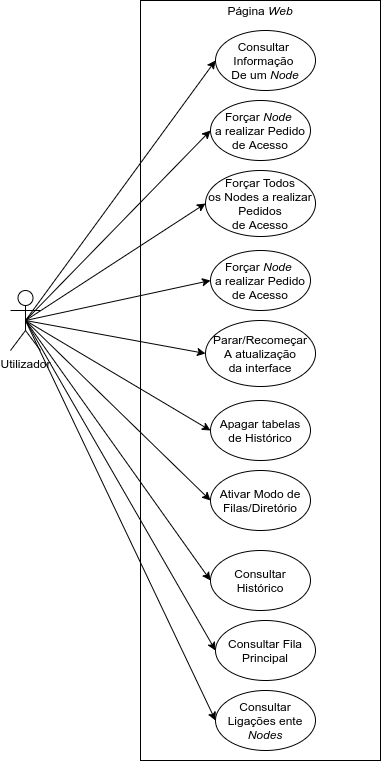
\includegraphics[width=250pt]{use_case_diagram.png}
\caption{Diagrama de Casos de Uso da Interface de Visualização.}
\label{engenharia:img:casos_de_uso}
\end{figure}

\begin{figure}[ht]
\centering
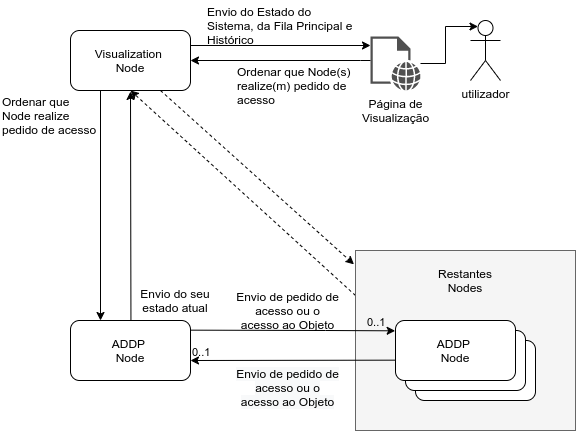
\includegraphics[width=400pt]{arquitetura.png}
\caption{Arquitetura do Sistema.}
\label{engenharia:img:arquitetura}
\end{figure}

\begin{figure}[ht]
\centering
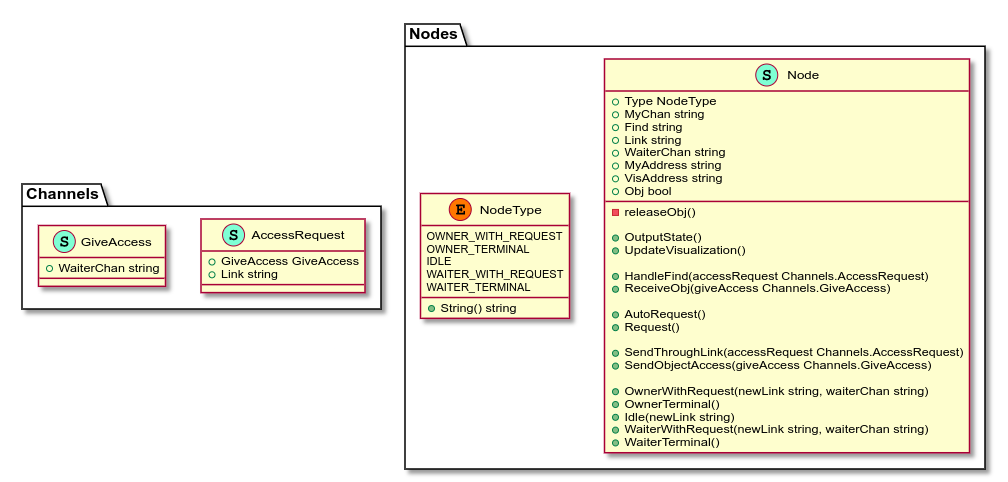
\includegraphics[width=400pt]{node_class_diagram.png}
\caption{Diagrama da Classe ``\emph{Node}''.}
\label{engenharia:img:classe}
\end{figure}




\section{Conclusão}
\label{engenharia:sec:conclusão} recebem o acesso ao objeto.
Neste capítulo foi exposta a o porquê da da mudança do projeto de um programa concorrente para um sistema distribuído e as alterações que essa decisão implicou no trajeto do projeto,
os motivos que levaram à escolha da Linguagem \emph{Go}, o planeamento de uma visualização do protocolo e do sistema em execução para uma prova parcial
e de como seria implementada essa
mesma interface, o uso da ferramenta/tecnologia \emph{Docker} para o \emph{Deploy} do sistema, a escolha do método de comunicação entre os \emph{Nodes} e o modelo
do funcionamento do sistema.

